% Einleitung

% Funktion

% Zertifizierung
% - 

% Details zu Verschlüsselung
% - Key exchange 
%   - via assymetric cryptograppy
%   - via Diffie Hellman Kex


Da \ac{http} Kommunikation unverschlüsselt erfolgt besteht die Möglichkeit, dass ein Angreifer der sich in einer \ac{mim} Position befindet sensible Daten abgreifen kann.
Beispielsweise kann ein Angreifer in einem öffentlichen WLAN-Netzwerk wie es beispielsweise in Bahnen oder an einigen öffentlichen Plätzen zur Verfügung gestellt wird Datenverkehr abgreifen.
Dadurch können Login-Credentials, Session IDs oder Zahlungsdaten die in einem solchen Netzwerk ausgetauscht werden abgehört werden.
Um derartige Angriffe verhindern zu können existiert das verschlüsselte Protokoll \textbf{\ac{https}}.
Nahezu alle Webseiten werden inzwischen mit Hilfe des Protokolls ausgeliefert.

\begin{figure}[!hbt]
    \centering
    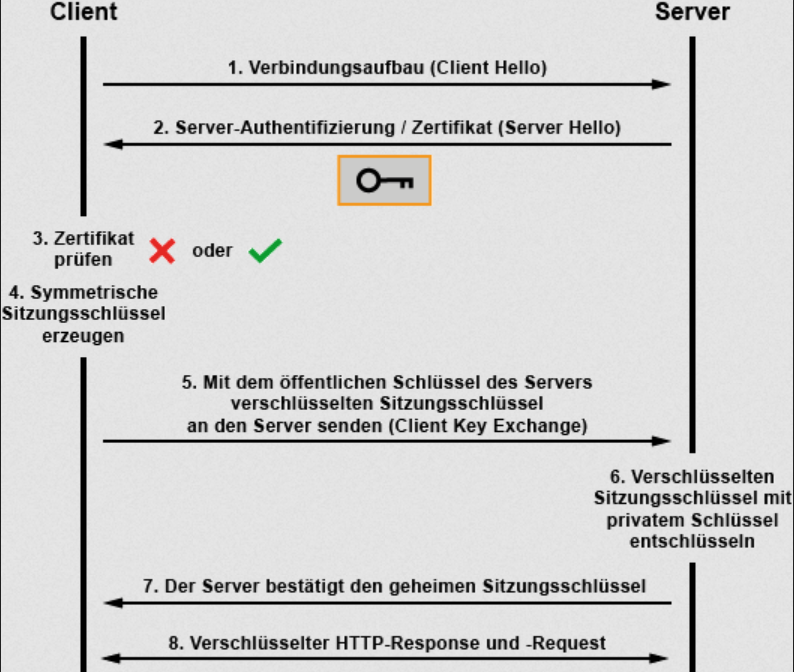
\includegraphics[width=0.7\textwidth]{./images/HTTPS-Processflow.png}
    \caption{Prozess Ablauf eines HTTPS Verbindungsaufbaus}
    \floatfoot{Quelle:\cite{HTTPSHTTPSecure}}
    \label{fig:https-porcess-flow}
\end{figure}

Die Aufgabe von \ac{https} ist, die Integrität und Vertraulichkeit der Kommunikation zwischen Webservern und Clients sicherzustellen.
Dies wird durch das Protokoll \ac{tls} umgesetzt das in der Lage ist die \ac{http} Kommunikation zu verschlüsseln.
\ac{tls} kann nicht ausschließlich im Rahmen von \ac{https} eingesetzt werden und kann beispielsweise auch zur Verschlüsselung von Mail-Kommunikation(SMTP) zum Einsatz kommen.
Der Ablauf des Verbindungsaufbaus und Zustandekommen der Verschlüsselung die bei \ac{https} zum Einsatz kommt ist in Abbildung \ref{fig:https-porcess-flow} schematisch dargestellt.

Der erste wichtige Vorgang ist, dass sich der Server, nachdem der Client eine Verbindung aufgebaut hat, mit einem TLS-Zertifikat bei den Client ausweist.
Der Client ist mit diesem Zertifikat in der Lage, die Identität des Servers zu überprüfen.
Dies erfolgt über eine Kette von Zertifikaten die sich hirarchisch bescheinigen authentisch zu sein.
Die mathematischen Prinzipien, die für dieses Verfahren notwendig sind sind für diese Thesis nicht relevant und werden nicht genauer betrachtet.
Nachdem der Client die Identität des Servers bestätigt ist es laut Protokoll auch möglich, dass sich der Client mit dem gleichen Verfahren beim Server authentifizieren kann, dies wird in der Realität jedoch äußerst selten vollzogen.\\

Hat der Server dem Client seine Identität bestätigt kann zwischen den Beiden einen Schlüssel ausgetauscht werden den beide Seiten nutzen können, um verschlüsselt kommunizieren zu können.
Um dies zu erreichen, ohne das eine etwaige dritte Person diesen Schlüssel Abhören und so die Kommunikation mitlesen kann erstellt der Client einen Schlüssel (shared secret).
Diesen übermittelt er dem Server asymmetrisch, mit dem öffentlich Schlüssel des Servers verschlüsselt.
Das \textit{shared Secret} kann nun ausschließlich mit dem privaten Schlüssel des Servers geöffnet werden.
Dieser Schlüsselaustausch kann auch mit den \textit{Diffie-Hellman} Verfahren ermittelt werden.
Dies ist zum Zeitpunkt eher selten.

Die Kommunikation zwischen Client und Server kann nun verschlüsselt stattfinden und nicht von einer dritten Person auf dem Weg abgefangen und verstanden werden.
Auch kann sich der Client sicher sein, direkt mit dem Server zu kommunizieren und das keine \ac{mim}-Attacke statt findet.

\pagebreak